\section{Basis for one-loop integrals} 
It is known that there exists a basis for one-loop integrals: one can write down an one-loop integral as linear combination of box (four-point), triangle (three-point), bubble (two-point) and tadpole (one-point) integrals (cf. figure~\ref{fig-mi}).
These integrals are called master integrals. 
In massless cases, they are however IR-divergent and we have to work in $D=4-2\epsilon$ dimensions.
\begin{figure}[h]
  \centering
  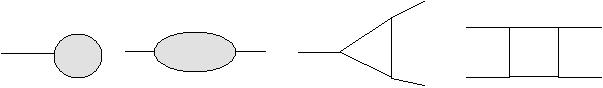
\includegraphics[width=0.5\linewidth]{master_integrals.jpg}
  \caption{Master integrals: tadpole, bubble, triangle and box}
  \label{fig-mi}
\end{figure}
Modern methods of one-loop amplitude computation are mostly based on the fact that we can decompose an amplitude in a basis with a finite number of integrals.
In massless cases, which we are most interested in, the tadpole integral vanishes. 
As a result, we can write an amplitude $A$ as
\begin{equation}\label{master_equation}
A = \sum_i c_i I_i + \mathrm{rational} + \mathcal{O}(\epsilon)
\end{equation}
where the $I_i$'s are box, triangle and bubble integrals and there may be finite polynomial term in kinematic invariants at the order of $\mathcal{O}(\epsilon^0)$.
Let us follow the review done in~\cite{Gluza:2010ws} on such a basis.
\\\\
We consider integrals in $D= 4-2\epsilon$ dimensions and keep external momenta to be four-dimensional.
A generic one-loop-integral can be written as
\begin{equation}\label{generic_loop_int}
I_n[P(l)] = 
-i\int\frac{\dd^D l}{(2\pi)^D}\frac{P(l)}{l^2(l-K_1)^2(l-K_{12})^2\ldots(l-K_{1\ldots n-1})^2}
\end{equation}
where $P$ is a polynomial in $l$.
Let us begin with integrals with high multiplicity, with five or more external legs.
In this case, we can use the Gram determinant defined as
\begin{equation}
\begin{split}
& G\begin{pmatrix}
p_1,\ldots, p_l \\
q_1,\ldots, q_l 
\end{pmatrix}
:= \det(2p_i\cdot q_j)
\\
& G(p_1, \ldots , p_l) := G\begin{pmatrix}
p_1,\ldots, p_l \\
p_1,\ldots, p_l 
\end{pmatrix}
\end{split}
\end{equation} 
to reduce the integral.
In fact, the Gram determinant vanishes if either $\{p_i\}$ or $\{q_i\}$ are linearly dependent.
One can expand each of the four-vectors $v^\mu$ in a basis $\{b_i\}_{i=1\ldots 4}$ composed of four chosen external momenta (\ie , the $K_i$'s in~\cref{generic_loop_int}) with the help of Gram determinants.
At one-loop, the terms $l\cdot b_i$ are reducible since we can write them as differences between terms appearing in the denominator of~\cref{generic_loop_int}.
They will lead to a sum of integrals with fewer propagators or fewer powers in $l$. 
In other words, 
\begin{equation}
I_n[(l\cdot v)^n] \rightarrow I_{n-1}[(l\cdot v)^{n-1}]\oplus I_n[(l\cdot v)^{n-1}]
\end{equation}
To prove our statement, we have to compute the contribution of five- or higher-point integrals with trivial numerator. 
We will show that they are of the order $\mathcal{O}(\epsilon)$.
Let us first consider the reduction of six- or higher-point integrals, which can be done to all orders in $\epsilon$. 
\\\\
Because the external momenta are taken in four dimensions,by the property of the determinant (external momenta are denoted only by numbers) 
\begin{equation}
G\begin{pmatrix}
l & 1 & 2 & 3 & 4\\
5 & 1 & 2 & 3 & 4 
\end{pmatrix}
 = 0
\end{equation}
Accordingly, by~\cref{generic_loop_int}
\begin{equation}\label{gram_induction}
I_n\Big[G\begin{pmatrix}
l & 1 & 2 & 3 & 4\\
5 & 1 & 2 & 3 & 4 
\end{pmatrix}\Big]
 = 0
 \quad\mathrm{for}\quad n\geq 6
\end{equation}
We can expand the Gram determinant appearing in~\cref{gram_induction} into a linear combination of Gram determinants of lower order (two arrays of four vectors instead of five).
The coefficients appearing in this expansion are either of the form $(l-K_i)^2$ or $K_i$, the external momenta.
\color{red} Maybe put the expression in an Appendix ?\color{black}
As a result,~\cref{gram_induction} will give us a relationship between an $n$-point integral and $(n-1)$-point integrals.
\\\\
As for the five-point scalar integral, there might be a worry about the $\mathcal{O}(\epsilon^0)$ term or even the divergent terms.
However, divergences appear only when the loop momentum $l$ is soft or collinear to one of the external momenta according to~\cref{generic_loop_int}, where the five-point Gram determinant also vanishes. 
We conclude that
\begin{equation}
I_5[G(l,1,2,3,4)] = \mathcal{O}(\epsilon)
\end{equation}
Hence, the five-point integral can also be reduced by expanding the Gram determinant into the lower order ones.
The reduction of five- or higher-point integrals are given explicitly in~\cite{Gluza:2010ws}.
%
%





